\newpage
\subsection{Method Signatures}
\texHeader
\hypertarget{static:methods tex}{}

\begin{itemize}

\item[$\blacktriangleright$] We're nearing the end of our model creation! One of the last things we need to do is to make the program \emph{do} something. After
all, what good is a program that only stores attributes and references?

\item[$\blacktriangleright$] Let's set up the operations we want each class to do by declaring their \emph{signatures}, starting with the
\texttt{Partition} class. We want a partition to be able to do three things: compare the answer on a \texttt{Card} with a guess and return a true/false
response, remove a specific card from that space, or empty itself of all cards.

\item[$\blacktriangleright$] Start with the \texttt{empty} method - it won't need any parameters, and it doesn't need to return anything. Declare this via an
\texttt{empty():void} command.

\item[$\blacktriangleright$] Create two more functions for \texttt{Partition} the same way. We'll need a \texttt{removeCard} method that accepts and returns a
\texttt{Card}, as well as a EBoolean \texttt{check} method that accepts a \texttt{Card} and an \texttt{EString} guess. 

\item[$\blacktriangleright$] Your partition class should now resemble Fig.~\ref{fig:partitionMethods}.

\vspace{0.5cm}

\begin{figure}[htbp]
	\centering
  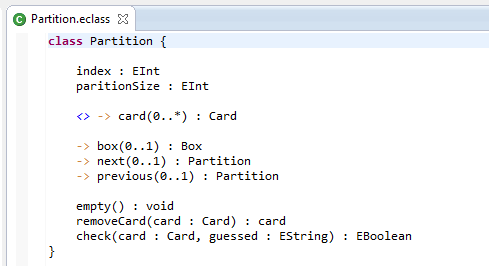
\includegraphics[width=0.6\textwidth]{eclipse_partitionMethods}
	\caption{The completed \texttt{Partition} class}
	\label{fig:partitionMethods}
\end{figure}

\vspace{0.5cm}

\item[$\blacktriangleright$] What needs to be done in the \texttt{Card} class? Well, in order to check the card, we'll need to be able to look at the flip side.
We'll also need to print whatever is on the current side. Create two paramater-less void functions, \texttt{invert} and \texttt{printCard}. 

% \item[$\blacktriangleright$] Your card class should now resemble Fig.~\ref{fig:cardMethods}
% 
% \begin{figure}[htbp]
% 	\centering
%   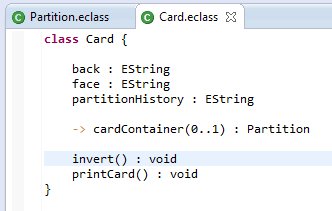
\includegraphics[width=0.5\textwidth]{eclipse_cardMethods}
% 	\caption{The completed \texttt{Card} class}
% 	\label{fig:cardMethods}
% \end{figure}

\clearpage

\item[$\blacktriangleright$] Finally, what do we need to do with the largest object in our model, the \texttt{Box}? In summary, we want a \texttt{Box} to:

\begin{description}
	{\small
  \item[\texttt{determineNextSize():EInt }] Find out how large the upcoming partition is
  \item[\texttt{grow():void}] Increase in size to allow more partitions
  \item[\texttt{toString():EString}] Translate the object attributes into strings
  \item[\texttt{addToStringRep(card:Card):void}] Print out all current content in the box
  }
\end{description}

\item[$\blacktriangleright$] Implement the above signatures, and your entire workspace should now resemble Fig.~\ref{fig:workspaceMethods} ({\small next page}).


\begin{figure}[htbp]
	\centering
  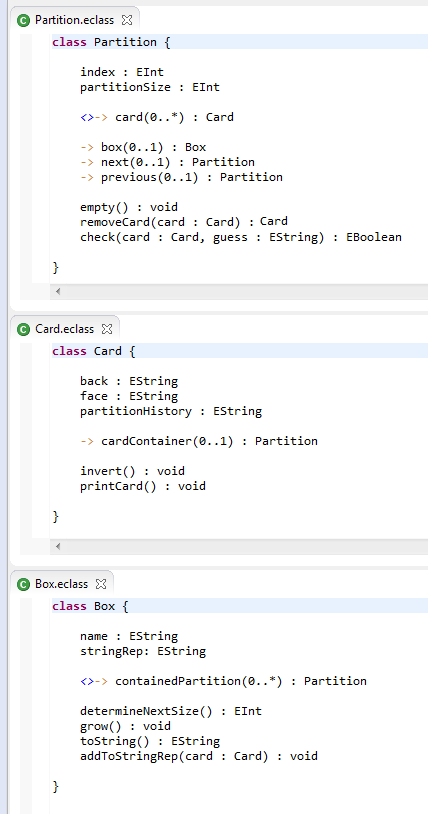
\includegraphics[width=0.7\textwidth]{eclipse_classesFullyDeclared}
	\caption{Completed method signatures}
	\label{fig:workspaceMethods}
\end{figure}

\item[$\blacktriangleright$] Congratulations! You have now created a full Learning Box type graph using eMoflon's textual syntax! To see how
this appears in the visual syntax, check out Fig.~\ref{fig:metamodel_complete} from the previous section. As a final step, build the project and wait for the
package explorer to refresh. 

\item[$\blacktriangleright$] Examine the generated files in ``gen'', especially the default implementation for those methods that just throw an
\texttt{OperationNotSupported} exception. We shall see in later parts of this handbook that the EMF code generator actually supports injecting hand-written
implementation of methods into generated methods and classes. With eMoflon however, we can model a large part of the dynamic semantics with ease, and only
need to implement small helper methods (such as those for string manipulation) by hand.

% \fancyfoot[R]{ $\triangleright$ \hyperlink{static review}{Next}}

\end{itemize}